%roll number 66 RISWANA T R

\textbf{\textcolor{LightMagenta}{Define the terms Hypothesis space and Version space. Illustrate with an 
example. (May 2019) \hfill 4 marks}}
\\[5pt]
{\textcolor{purple}{Hypothesis space:}}\\
For a binary classification problem , There may be more than one hypothesis present, such a set of hypothesis is called a hypothesis space.\\


\graphicspath{ {./} }
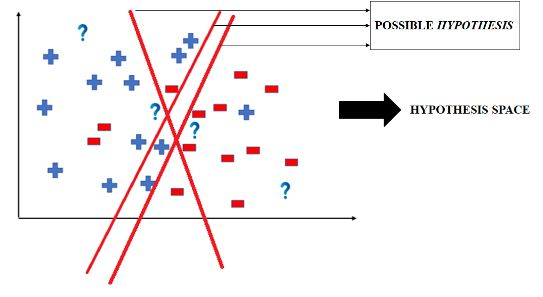
\includegraphics{Images/A23_img1.JPG}\\
{\textcolor{purple}{Consistency:}}\\
Let 'x' be an example of classification problem and C(x) denote the class label to ,'x', i.e, C(x) = 1 or 0.\\
\\
Let  D be the training set; ‘h’ be the hypothesis for the problem, h(x) be the class label assigned to ‘x’ by h.\\
\\
h is consistent, if h(x) = C(x) , $\forall$ D.\\
\\
Example:
\\


 \begin{table}[h]                           
 \centering
    \begin{tabular}{|c|c|}
    \hline
  \textcolor{purple}{Feature}   &    \textcolor{purple}{Class label}            \\ \hline
     27     &  1     \\ \hline          
     15     &  0 \\ \hline
     23     &  1   \\ \hline
     30     &  1    \\ \hline
     25     &  1  \\ \hline
     17     &  0   \\ \hline
     12     &  0 \\ \hline
     31     &  1     \\ \hline
     6      &  0   \\ \hline

    \end{tabular}
    \label{tab:msg1}                            

\end{table}\\

$$
 \left.
    \begin{array}{ll}
  \mbox{h1 If  x  $>$ 17 then 1 else 0 }        \\
  \mbox{h2  If  x $\geq$ 18 then 1 else 0 }     \\
  \mbox{h3 If  x $\geq$  20 then 1 else 0}      \\
  \mbox{h4 If  x  $\geq$ 23 then 1 else 0}
  \end{array}
\right \}\mbox{Hypothesis space}
$$

\\
\\
{\textcolor{purple}{Version space:}}
\\
Consider a binary classification problem ,
Let D be the data set ,H be the Hypothesis space,Then version space of the problem with respect to D and the space H consistent with D,i.e,\\
VS$_{D,H}$ = \{ h $\in$  H ,h(x)=C(x) \}\\
\\

Example:
 \begin{table}[h]                           
 \centering
    \begin{tabular}{|c|c|c|}
    \hline
  \textcolor{purple}{x1}    &  \textcolor{purple}{x2} &    \textcolor{purple}{Class label}            \\ \hline
  6      &   8    & +1         \\ \hline          
     12    &  14  & -1 \\ \hline
      3   &   2   & +1      \\ \hline
     18    &   17 & -1        \\ \hline

    \end{tabular}
    \label{tab:msg1}                            

\end{table}\\

h1 if  x1 $<$ 10 and X2 $<$ 10  then +1 else -1\\
h2 if x1+x2 $<$ 15 then +1 else -1\\
h3 if x1 $>$ 10 And  x2 $>$ 10 then -1 else +1\\
\\
Collection of consistent hypothesis is called version space.